\chapter{Graphical User Interface}
\renewcommand{\kapitelautor}{Autor: Andreas Novak}

\section{Einleitung}
Mit dem Gedanken, dass ein Dateisynchronisationstool hauptsächlich im
Hintergrund arbeitet, ist die grafische Benutzeroberfläche zurückhaltend und
einfach gestaltet. Dem Nutzer werden nicht unnötig viel
Konfigurationsmöglichkeiten gegeben, damit er leicht den Überblick behalten
kann. Beim Starten von sblit erscheint das Icon im System-Tray, welches als
Angelpunkt für jegliche Nutzerinteraktion dient.

\section{Überblicksfenster}
%\begin{figure}[H]
	\centering
	\includegraphics[scale=0.7]{images/ueberblicksfenster.png}
  \caption{Überblicksfenster}
	\label{ueberblicksfenster}
\end{figure}

Mit einem einfachen Klick auf das Icon im System-Tray öffnet sich das Überblicksfenster, in der der
Benutzer auf die folgenden Optionen Zugriff bekommt:

\begin{description}

	\descriptionitem{Letzte Änderungen innerhalb des sblit-Ordners}
		Dem Benutzer wird hier eine Auflistung der zuletzt hinzugefügten Dateien
		geboten. Neben dem an den Dateityp angepassten Bild wird auch der Dateiname
		und Ordnerpfad angegeben.

	\descriptionitem{Fortschrittsbalken laufender Synchronisationsvorgänge}
		Bei laufenden Synchronisationen hat der User die Möglichkeit, den
		Fortschritt zu verfolgen.

	\descriptionitem{Button für das Abbrechen der Synchronisation}
	  Beispielsweise nach irrtümlichem Hinzufügen von Dateien, hat der Benutzer die
		Möglichkeit, die laufende Synchronisation mithilfe des Abbrechen-Buttons
		abzubrechen.

	\descriptionitem{Anzeige von aufgetretenen Fehlern}
		Bei \glspl{syncconflict}n, die auftreten, wenn zwei \glspl{syncpartner} die
		selbe Datei gleichzeitig bearbeiten, sowie bei diversen anderen Fehlern,
		wird der User benachrichtigt.

	\descriptionitem{Link zum sblit-Ordner}
		Um dem Benutzer schnellen Zugriff auf seinen konfigurierten sblit-Ordner zu
		gestatten, gibt es den Ordner-Button, mit dem sich der sblit-Ordner im
		Datei-Browser öffnet.

	\descriptionitem{Öffnen des Konfigurationsmenüs}
		Mit einem Klick auf den Optionen-Button öffnet sich das Konfigurationsmenü,
		welches im folgenden Abschnitt gezeigt wird.
\end{description}


\section{Konfigurationsmenü}
%\begin{figure}[H]
	\centering
	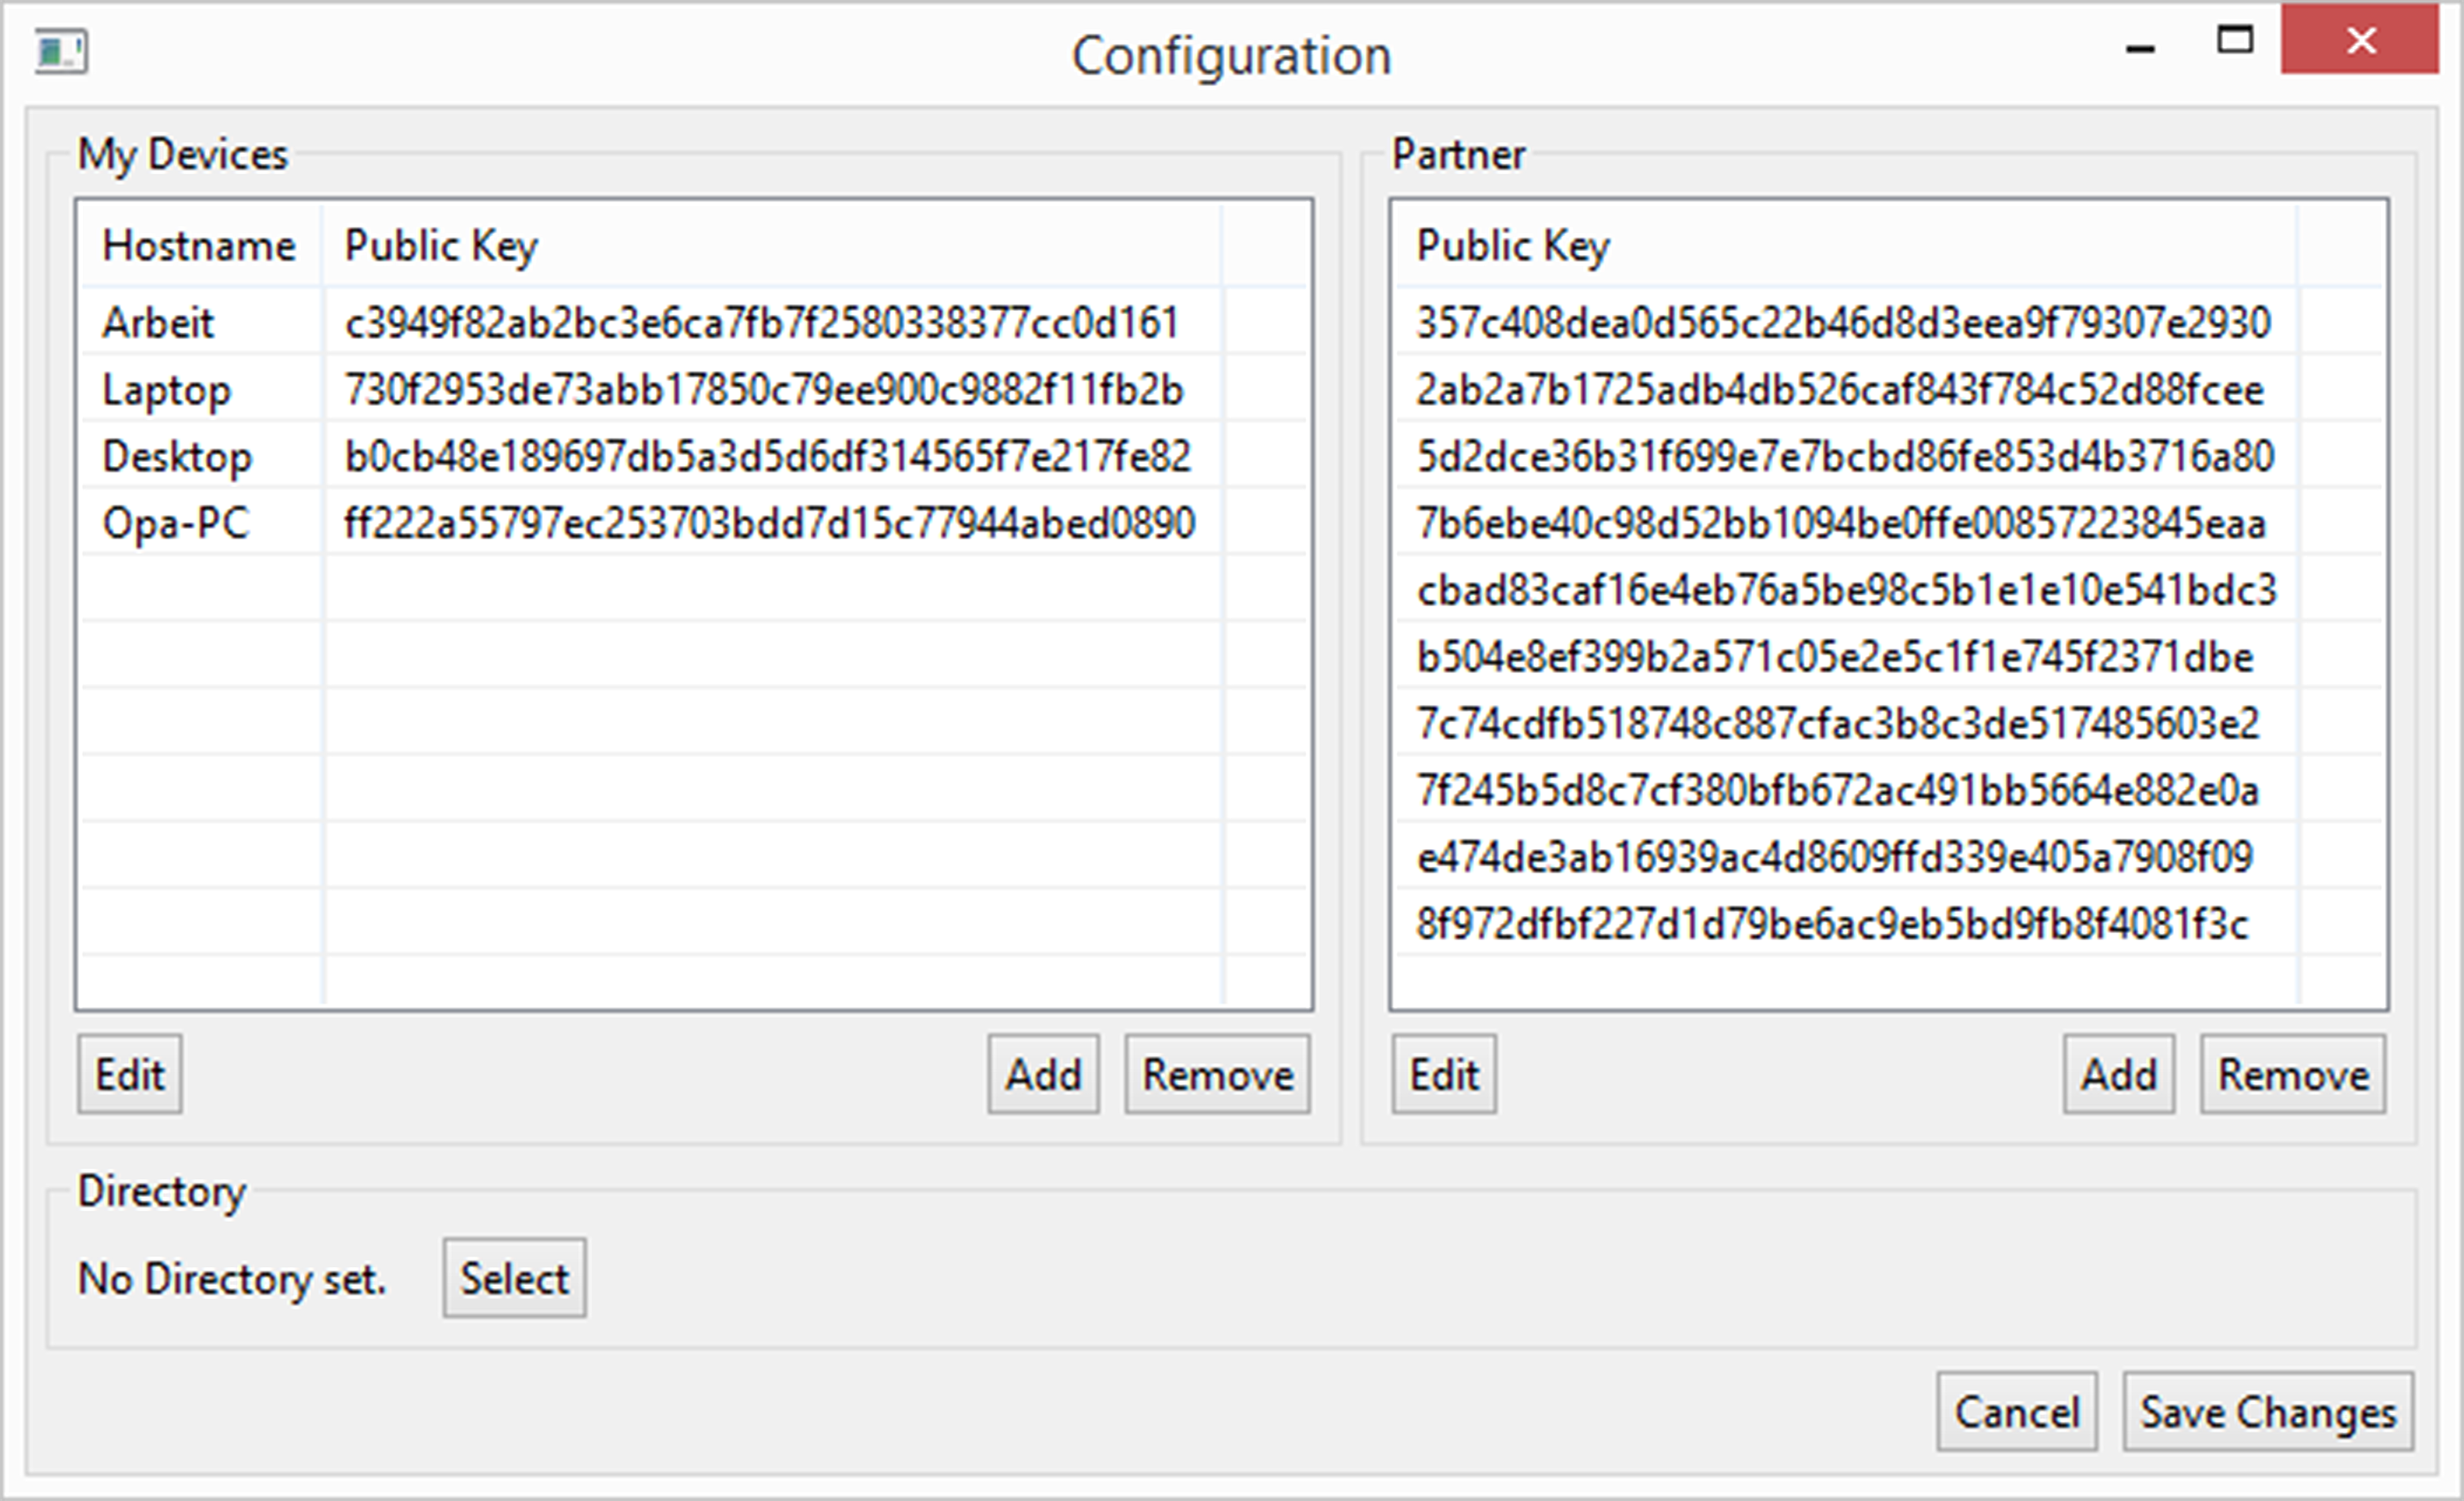
\includegraphics[]{images/config_gui.jpg}
	\label{config_gui}
  \caption{Konfigurationsmenü}
\end{figure}
\begin{description}

	\descriptionitem{Geräte zu den Synchronisationspartnern hinzufügen/entfernen}
		Unter dem Punkt “My Devices” befindet sich die Liste der
		Synchronisationsgeräte, also jene Geräte, mit denen der unter Punkt 3
		angegebene sblit-Ordner synchronisiert wird. Die Einträge
		bestehen aus dem vom Benutzer angegebenen Namen des Geräts und dessen
		Public-Key, welcher seine Adresse darstellt. Der Benutzer hat die
		Möglichkeit, bestehende Einträge für Korrekturen zu bearbeiten, neue
		hinzuzufügen oder alte zu entfernen.

	\descriptionitem{Manuelles Eintragen von Partnergeräten}
		Obwohl die Liste der Partnergeräte automatisch von \sblit verwaltet wird,
		hat der Benutzer die Möglichkeit, Geräte manuell hinzuzufügen. Während
		nämlich normalerweise Geräte fremder Nutzer als Partnergeräte fungieren,
		kann man sich auch gegenseitig mit einer Freundin oder einem Freund
		Speicherplatz freigeben, indem man den Public-Key des jeweils anderen in der
		Liste der Partnergeräte einträgt.

	\descriptionitem{Verschieben des sblit-Ordners}
		Der zu synchronisierende Ordner kann im Konfigurationsmenü auch nach der
		Installation noch geändert und verschoben werden.

\end{description}

